\chapter{Corpus Creation}

One of the steps of the analysis of the prevalence of the dark pattern on Czech webshops is to find webshops URLs on a large scale autonomously. The Princeton researchers used Alexa Rank\cite{alexa-topsites} made by a web traffic analysis company, Alexa Internet. Alexa Rank is a measure of website popularity. Alexa Internet provides API to fetch a list of most popular websites by Alexa Rank. However, this list contains other types of websites as well, not only webshops that researchers focus on. Also, non-English websites are included as well. Because of that, researchers implemented a couple of mechanisms to cherry-pick English webshops only, discussed earlier in the state-of-the-art chapter of this thesis.

As said before, this thesis aims to analyse Czech webshops and because of that, using Alexa Rank is not efficient enough. Alexa API provides only the first five hundred thousand most popular websites, which is a reason why it contains a small number of Czech websites and even fewer Czech webshops. However, the Czech Internet (that means only websites in the Czech language) is relatively small compared to the English Internet. Also, the English Internet is under multiple jurisdictions, but the Czech Internet is not. Therefore, the Czech Internet is more consistent, and a result of it is that this environment allows creating companies that make Internet catalogues and comparison shopping websites (aggregators) that cover a significant portion of the Czech Internet. 

These catalogues and tools also sometimes rank the listed websites by a measure that has connotations to popularity. For example, a number of testimonials are an excellent resource that reflects the popularity of the webshop. These catalogues and aggregators can be used to mine the URLs of Czech webshops from them instead of using Alexa Rank API. Also, if there is a similar measure as described above, the analysis results can be compared to Princeton's researcher analysis, revealing a correlation of dark patterns evidence on the website and the popularity of the website.

While searching the Internet, several such suitable sites were discovered that contain extensive lists of Czech webshops. Examples of the most suitable sites are Heureka.cz, Asociaceeshopu.cz and Shopy.cz.

Other vital facts that played a role and were considered in the selection of the only one website (that is later used for the creation of the list of Czech webshops) were the actual cover of the Czech Internet. Heureka has by far the highest number of webshops in their listings\cite{srovnavace-shoptet}. However, a few of the biggest webshops do not want to be listed on Heureka. Their reason is usually Heureka itself because it compares the prices of products on the enlisted webshops. Also, Heureka is a part of a business group that runs several competitive webshops. Because of that, the final list (made in this practical part of the study) of Czech webshops was manually checked if it contains the five biggest webshops (according to the list published on website peak.cz\cite{peak-eshopy}), and it does.

\begin{figure}[ht]
    \centering
    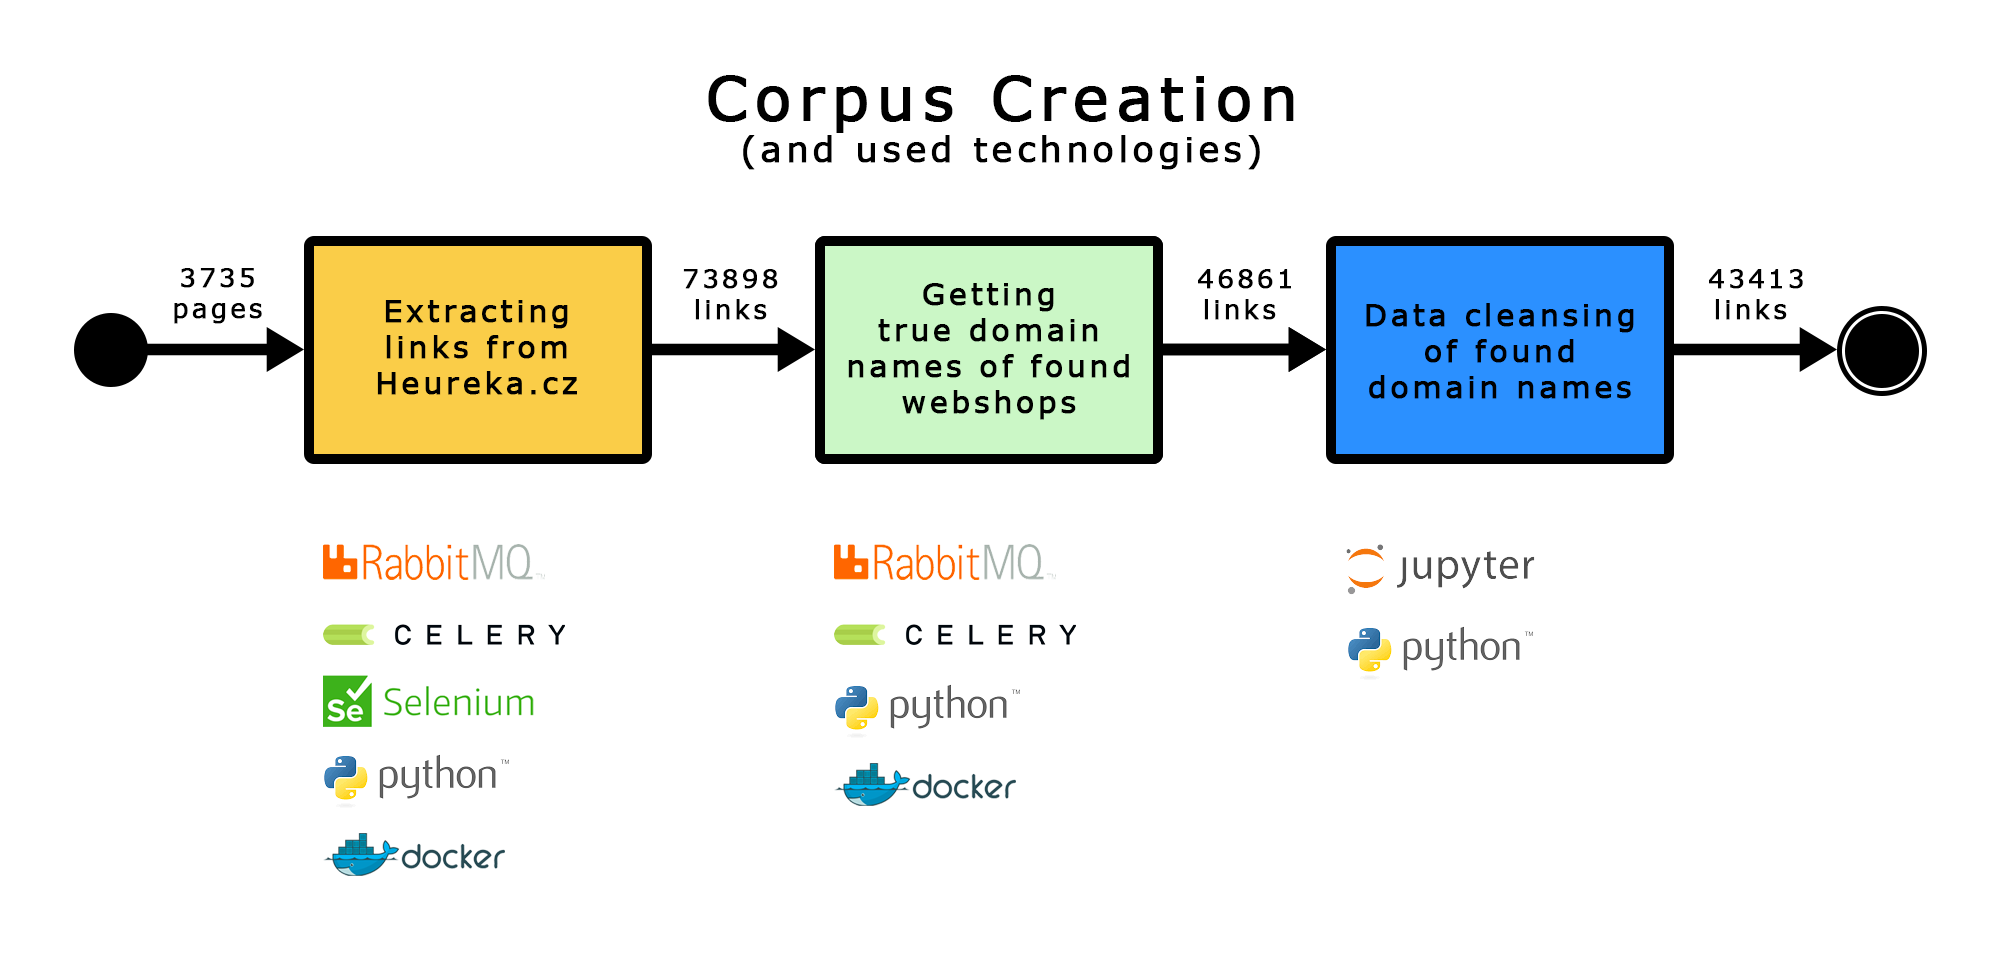
\includegraphics[width=1\linewidth]{media/corpus_creation.png}
    \caption{All steps of corpus creation, which starts with a list of webshops available on Heureka.cz, paginated into 3735 pages and ends with a list of 43413 unique webshops' URLs in CSV format.}
    \label{fig:corpus_creation}
\end{figure}

\section{Extracting webshops from Heureka}

Heureka provides a list of all registered webshops on their website. This list is paginated, where every page contains twenty records of webshops. However, Heureka does not provide the total number of these pages. 

In February 2021, the total number of pages was 3735. This number of pages was manually found by changing the query parameters from the URL until the page stopped returning error 404. At the same time, these 3735 pages contained 74698 webshops in total. 

A web crawler was made to extract webshops' links and names from these pages. The crawler is written in Python 3, using Selenium framework with Chrome browser in headless mode. Also, the crawler is parallelised to speed up this task using Celery asynchronous task queue. Source codes are inside \textbf{src\string/crawler\string/extract\_shops} folder. 

Some of the crawled pages were not successfully downloaded because the Chrome browser occasionally failed to start or the webserver returned an empty page. The crawler was still able to successfully download \textbf{3695 pages} containing \textbf{73898 webshops} in total after scraping the HTML into 3695 CSV files.

Such a high number of obtained webshops does not correspond with the number of webshops that Heureka claims to contain on its homepage (it claims to aggregate around 38000 webshops). Also, the estimated number of webshops on the Czech Internet is around 41000 according to a study made by Zbozi.cz and Shoptet.cz\cite{srovnavace-shoptet}. The cause of this is that the retrieved list of webshops contains many duplicities and already inactive webshops.

Another problem with this list is that the retrieved links are not the actual domain names of the webshops. These URLs are redirections, and they must be visited first to retrieve the actual domain name.

The two other steps of the Corpus Creation deal with these two problems.

\section{Retrieving true domain names}

As mentioned above, Heureka does not provide direct URLs to webshops in its listings. The provided links only redirect to the true URLs of webshops, and because of that, another crawler was made to follow these redirections and return the true URLs. This crawler is also written in Python 3. This time, the task is only to retrieve the true URLs. Hence, Request library is used instead of Selenium, which is too complex for such a simple task. It remains parallelized using Celery. Sources codes are in \textbf{src\string/crawler\string/reveal\_true\_domains} folder.

This crawler adds an additional column to the dataset given from the previous crawler, which contains the true URL. If an exception occurred during the execution of the single task, its message is written there instead. If the webpage returned a different status code than 200, the status code is also written there instead. The importance of this data about errors and exceptions are helpful in the validation of the whole task. Whether the whole task is successful or it returns too many errors and exceptions.

\section{Cleansing of dataset}

The given data from the previous crawler is further cleansed in a Jupyter notebook \textbf{src\string/crawler\string/domain\_dataset\_cleansing.ipynb} using primarily Pandas library.

In the first step, the dataset is split into two data frames of errors and true URLs. Dataset of errors contains 27037 rows, and 23238 of them are results of connection being refused after redirection. The first exception might be that Heureka implemented mechanisms to prevent the crawling of the redirections. This claim was refuted by \textbf{manually going through 100 random} links. None of these links redirects to an active webshop. The next most frequent errors were 404 errors with 1953 occurrences, 403 errors with 750 occurrences and 503 errors with 504 occurrences. These are errors that indicate that the web store web page is no longer active. The other errors had an incidence of fewer than 200 occurrences.

The dataset of true URLs is further cleansed by filtering out other identified inactive webshops that were not identified in the error/rejection filtering. Firstly, such webshops URLs have a high frequency in the dataset because the webshops' URLs are often redirected to the webshops' hosting service website after deactivation of the webshop. For example, many Czech webshops use Shoptet service, which allows users to rent a done webshop solution for a monthly payment. After the users stop paying this fee, their webshop is inactivated (or deleted), making the original webshop be redirected to Shoptet's custom webpage informing visitors about the inactivation of the particular webshop. Secondly, many URLs of inactive webshops contain status code in the URL without sending the actual status code in an HTTP response. Lastly, some domain names were inactive or resold and redirected to a new website (surprisingly redirected to porn websites in most of the cases). All this manual work led to creating a list of such URLs and was used to filter them out of the dataset. This shrinked the dataset from \textbf{46861} to \textbf{46023} rows, removing another \textbf{838} rows.

The last step is to remove URI parts from the URLs and drop duplicate entries, which shrank the dataset to final \textbf{43413} unique links to webshops, removing another \textbf{2610} rows.

Links to download all the outputs and logfiles of crawling are on README page of GitHub repository of this thesis. The link to this repository is in Appendix B (Supplemental Material) of this thesis.

The final list of Corpus Creation stage can be found \textbf{clean\_eshop\_list.csv} in an archive \textbf{reveal\_true\_domains\_crawl\_2021\_02\_23.tar.bz2}.

% dát tam tabulčičku, která to zesumíruje